\chapter{Diseño del Sistema y Arquitectura}
\label{cap:diseno}

Este capítulo describe la arquitectura de SGROAS, las decisiones de diseño documentadas como ADR, el modelo de datos, el diseño de la API REST y la matriz de trazabilidad con la columna adicional \texttt{tipo\_acceso}.

\section{Arquitectura general}
\label{sec:arquitectura-general}

SGROAS adopta una arquitectura monolítica de tres capas \cite{martin2017}, documentada con el modelo C4 \cite{c4model} en los niveles 1--3 mediante Structurizr DSL (archivos en \texttt{docs/arquitectura/}).

\subsection{Contexto (C4 nivel 1)}

El sistema interactúa con tres actores principales (Administrador, Coordinador, Personal de Seguridad) y se conecta a dos sistemas externos: PostgreSQL 16 (base de datos transaccional) y Redis 7 (caché distribuida y blacklist de JWT).

\begin{figure}[H]
  \centering
  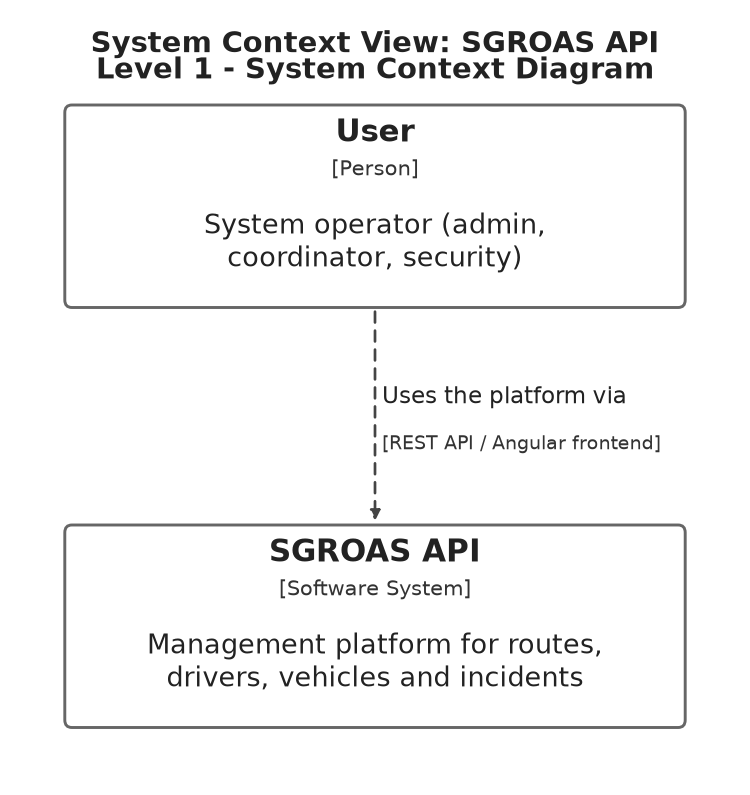
\includegraphics[width=0.85\textwidth]{c4-level1-context.png}
  \caption{C4 Level 1 Diagram --- SGROAS System Context.}
  \label{fig:c4-level1}
\end{figure}

\subsection{Contenedores (C4 nivel 2)}

El sistema se compone de cuatro contenedores:
\begin{itemize}
  \item \textbf{Frontend (Angular 20):} SPA que consume la API REST. Desplegado como parte del backend (compilado con \texttt{ng build} y servido desde \texttt{src/main/resources/static/}).
  \item \textbf{Backend (Spring Boot 3.5.x / Java 21 LTS):} API REST con controladores, servicios y repositorios. Empaquetado como JAR ejecutable.
  \item \textbf{PostgreSQL 16:} Base de datos relacional con migraciones Flyway.
  \item \textbf{Redis 7:} Caché distribuida para listados paginados y blacklist de JTI.
\end{itemize}

\begin{figure}[H]
  \centering
  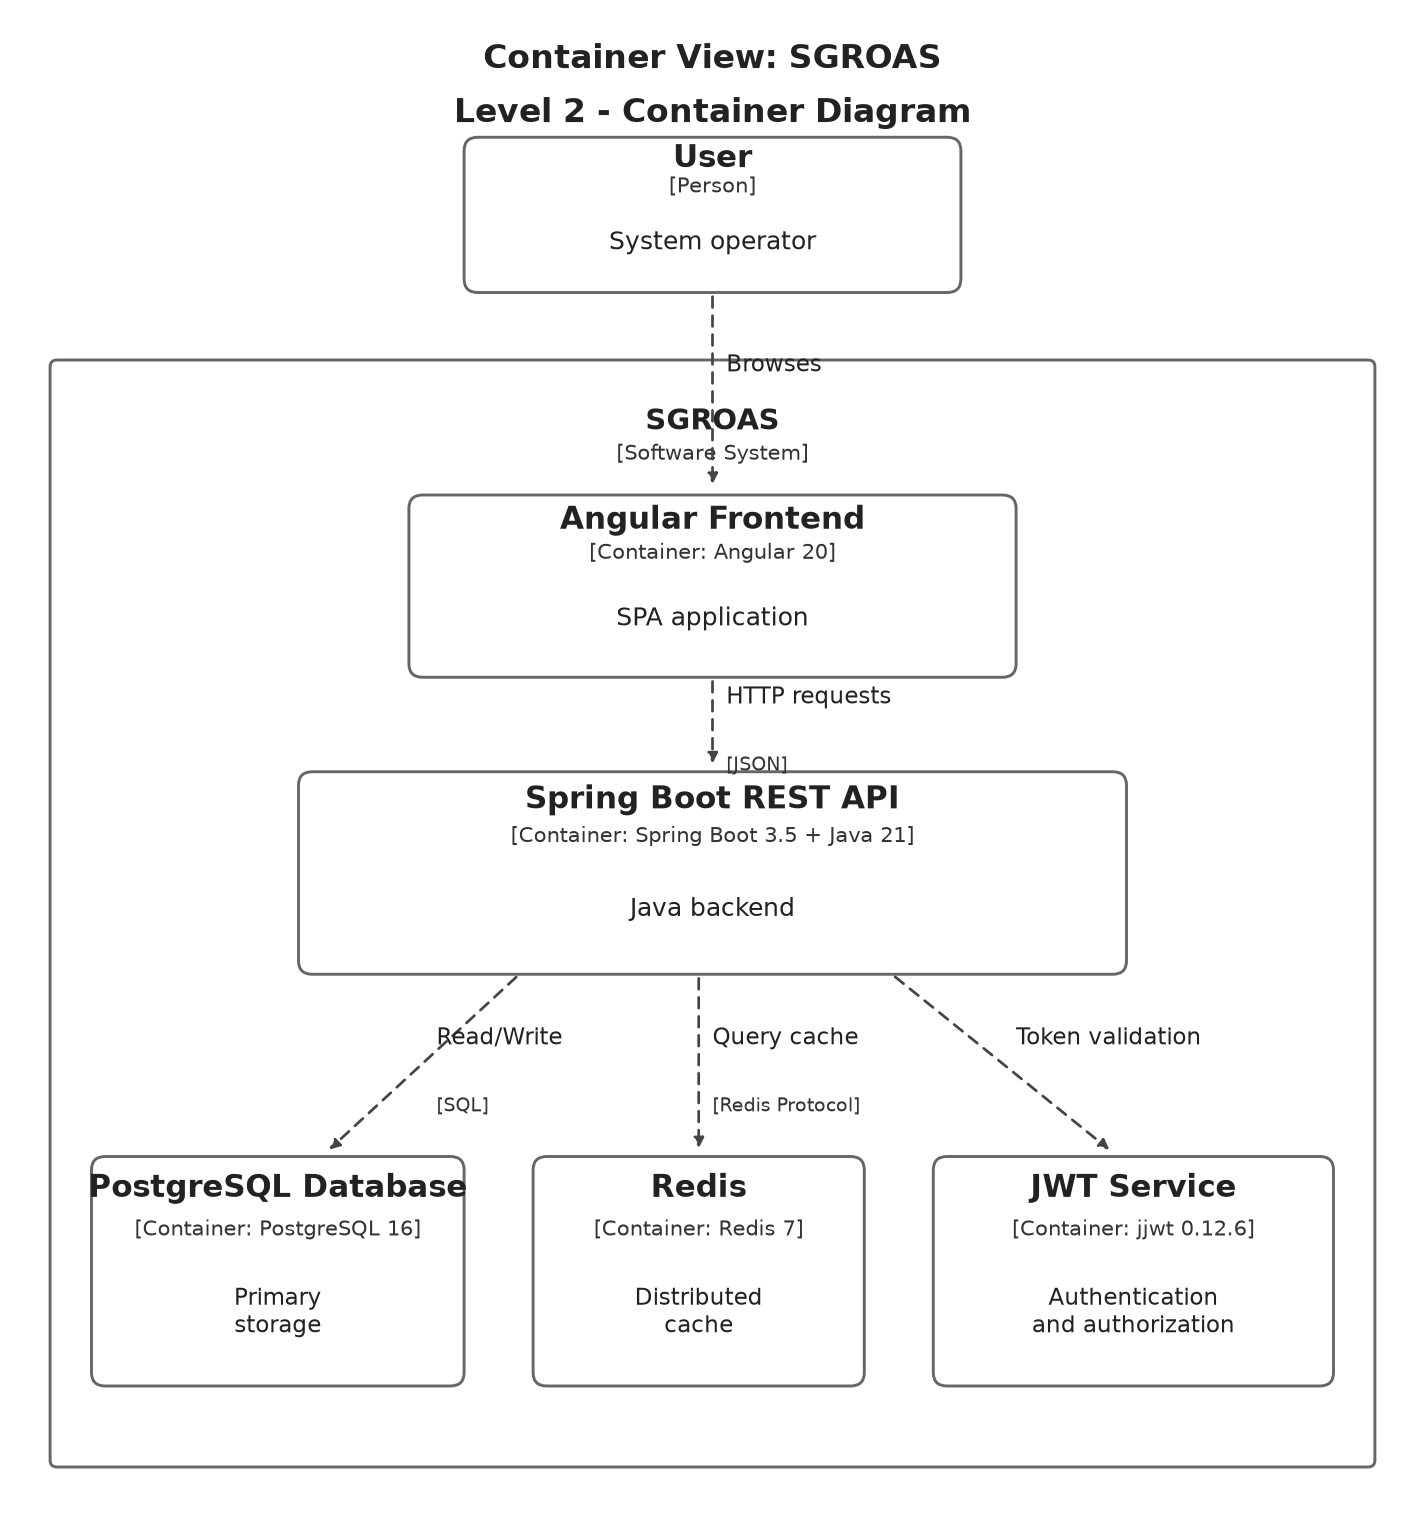
\includegraphics[width=0.85\textwidth]{c4-level2-containers.png}
  \caption{C4 Level 2 Diagram --- SGROAS System Containers.}
  \label{fig:c4-level2}
\end{figure}

\subsection{Componentes (C4 nivel 3)}

El backend se organiza en paquetes:
\begin{itemize}
  \item \texttt{ec.edu.uteq.sgroas.controller}: controladores REST (\texttt{AuthController}, \texttt{ConductorController}, \texttt{UsuarioController}, \texttt{RutaController}, \texttt{VehiculoController}, \texttt{AsignacionRutaController}, \texttt{IncidenteController}).
  \item \texttt{ec.edu.uteq.sgroas.service}: lógica de negocio (\texttt{AuthService}, \texttt{ConductorService}, \texttt{ReporteService}).
  \item \texttt{ec.edu.uteq.sgroas.repository}: repositorios Spring Data JPA.
  \item \texttt{ec.edu.uteq.sgroas.entity}: entidades JPA con \texttt{@NamedStoredProcedureQuery}.
  \item \texttt{ec.edu.uteq.sgroas.dto}: DTOs como Java Records.
  \item \texttt{ec.edu.uteq.sgroas.config}: configuración de seguridad, caché y CORS.
\end{itemize}

\begin{figure}[H]
  \centering
  \includegraphics[width=0.85\textwidth]{c4-level3-components.png}
  \caption{C4 Level 3 Diagram --- SGROAS Backend Components.}
  \label{fig:c4-level3}
\end{figure}

\section{Decisiones de Arquitectura (ADR)}
\label{sec:adr}

El repositorio contiene ocho ADRs siguiendo la plantilla de Nygard \cite{nygard2017}. Los siete obligatorios se resumen a continuación.

\subsection{ADR-001: Arquitectura monolítica con Spring Boot}

Se adopta una arquitectura monolítica porque el equipo es pequeño (3 integrantes) y el dominio es acotado. La alternativa de microservicios con Spring Cloud se descartó por sobreingeniería. Consecuencia: simplicidad de despliegue y monitoreo; riesgo de acoplamiento a largo plazo.

\subsection{ADR-002: JPA + Hibernate con Flyway para persistencia}

JPA + Hibernate como ORM con \texttt{ddl-auto=validate} y Flyway para migraciones versionadas. La alternativa de \texttt{ddl-auto=update} se descartó por riesgos en producción. Consecuencia: esquema versionado y reproducible.

\subsection{ADR-003: Autenticación stateless con JWT}

JWT con access tokens (1 hora) y refresh tokens (7 días) según RFC 7519 \cite{rfc7519}. El token se almacena en cookie HttpOnly + Secure + SameSite=Strict. Las alternativas de sesiones HTTP y OAuth2 con Keycloak se descartaron por requerir estado en servidor y sobreingeniería, respectivamente.

\subsection{ADR-004: Cache distribuido con Redis}

Redis como caché de segundo nivel para listados paginados frecuentes (\texttt{@Cacheable} / \texttt{@CacheEvict}). La alternativa de Caffeine (caché en memoria) se descartó por no compartirse entre instancias.

\subsection{ADR-005: Diseño de base de datos con soft delete}

Soft delete (columna \texttt{activo} booleana) en todas las tablas, llaves foráneas con \texttt{ON DELETE RESTRICT}, y triggers para timestamps automáticos. La alternativa de hard delete se descartó por pérdida de trazabilidad.

\subsection{ADR-006: Estrategia híbrida de acceso a datos (CRUD-ORM + SP)}

\label{sec:adr006}

Este ADR documenta la decisión más relevante para la estrategia de acceso a datos. El sistema separa:

\begin{enumerate}
  \item \textbf{CRUD elementales:} Implementados con Spring Data JPA (\texttt{JpaRepository}) usando consultas derivadas de nombres de métodos. Sin \texttt{@Query} ni \texttt{createNativeQuery}.
  \item \textbf{Operaciones adicionales:} Agregaciones, reportes y validaciones encapsulados en stored procedures y funciones SQL de PostgreSQL, instalados por la migración Flyway \texttt{V5\_\_\_stored\_procedures.sql}.
\end{enumerate}

La invocación de stored procedures se realiza exclusivamente mediante \texttt{@NamedStoredProcedureQuery} declarada en la entidad + \texttt{@Procedure(name=...)} en el repositorio (mecanismo JPA 2.1). El cursor de salida se declara con \texttt{@StoredProcedureParameter(mode = ParameterMode.REF\_CURSOR, type = Class.class)}. Los REFCURSOR de PostgreSQL solo son legibles dentro de la misma transaccion JDBC, por lo que la capa de invocación (\texttt{ReporteService}) está anotada con \texttt{@Transactional}.

Las alternativas descartadas fueron: (1) \texttt{FUNCTION RETURNS TABLE} + \texttt{@Procedure} (Hibernate genera \texttt{CALL} que solo existe para \texttt{PROCEDURE}); (2) \texttt{PROCEDURE} + \texttt{outputParameterName} (Spring Data omite el parámetro de salida); (3) \texttt{PROCEDURE} + \texttt{@NamedStoredProcedureQuery} sin \texttt{REF\_CURSOR} (tipo incorrecto).

\subsection{ADR-007: Despliegue público en Render (PaaS)}

El sistema se despliega en Render con certificado TLS automático, PostgreSQL gestionada y autodeploy desde GitHub. La alternativa de VPS propio se descartó por operación manual fuera del alcance del equipo.

\section{Diseño de la base de datos}
\label{sec:diseno-bd}

El modelo de datos incluye las siguientes tablas principales:

\begin{itemize}
  \item \texttt{conductores}: cédula, nombre, licencia, fecha vencimiento, teléfono, email, activo.
  \item \texttt{usuarios}: email, contraseña (BCrypt), nombre, rol (enum: ADMIN, COORDINADOR, SEGURIDAD), activo.
  \item \texttt{rutas}: código, nombre, origen, destino, distancia, precio.
  \item \texttt{vehiculos}: placa, marca, modelo, año, capacidad, número disco, activo.
  \item \texttt{asignacion\_rutas}: relación conductor-vehículo-ruta con fechas de vigencia.
  \item \texttt{incidentes}: tipo, descripción, fecha, gravedad, estado, ubicación, relación con asignación.
  \item \texttt{alertas}: nivel de riesgo, descripción, fecha, relación con incidente.
  \item \texttt{programacion}: fecha, hora salida/llegada, estado, relación con ruta/unidad/conductor.
  \item \texttt{auditoria}: acción, fecha, IP, relación con usuario (trigger \texttt{trg\_auditoria\_alerta}).
\end{itemize}

Las migraciones se versionan con Flyway (\texttt{V1} a \texttt{V13}) en \texttt{src/main/resources/db/migration/}. El esquema se valida automáticamente con \texttt{ddl-auto=validate} al iniciar la aplicación.

\section{Diseño de la API REST}
\label{sec:api-rest}

La API sigue los principios de Fielding \cite{fielding2002} con los siguientes endpoints principales:

\begin{longtable}{@{}p{3.5cm}p{2cm}p{2.5cm}p{2.5cm}@{}}
\caption{Main REST API endpoints.}
\label{tab:api-rest}\\
\toprule
\textbf{Recurso} & \textbf{Método} & \textbf{Endpoint} & \textbf{Roles permitidos} \\
\midrule
\endfirsthead
\toprule
\textbf{Recurso} & \textbf{Método} & \textbf{Endpoint} & \textbf{Roles permitidos} \\
\midrule
\endhead
Autenticación & POST & /api/auth/login & Público \\
Autenticación & POST & /api/auth/refresh & Autenticado \\
Conductores & GET/POST & /api/conductores & ADMIN, COORDINADOR \\
Conductores & GET/PUT/DELETE & /api/conductores/\{id\} & ADMIN, COORDINADOR \\
Usuarios & GET/POST & /api/usuarios & ADMIN \\
Rutas & GET/POST & /api/rutas & ADMIN, COORDINADOR \\
Vehículos & GET/POST & /api/vehiculos & ADMIN, COORDINADOR \\
Asignaciones & GET/POST & /api/asignaciones & ADMIN, COORDINADOR \\
Incidentes & GET/POST & /api/incidentes & ADMIN, SEGURIDAD \\
Programaciones & GET/POST & /api/programaciones & ADMIN, COORDINADOR \\
Alertas & GET & /api/abd/alertas & ADMIN, SEGURIDAD \\
Reportes & GET & /api/reportes/* & ADMIN \\
Actuator & GET & /actuator/health & Público \\
\bottomrule
\end{longtable}

Los DTOs se implementan como Java Records inmutables (\texttt{ConductorRequest} / \texttt{ConductorResponse}) con validación Jakarta Validation (\texttt{@NotBlank}, \texttt{@Email}, \texttt{@Pattern}). El manejo global de excepciones se implementa con \texttt{@RestControllerAdvice} siguiendo RFC 7807 (Problem Details) \cite{rfc7807}.

\section{Matriz de trazabilidad}
\label{sec:matriz-trazabilidad}

La matriz de trazabilidad (\texttt{docs/trazabilidad/matriz.csv}) conecta cada requisito con su historia de usuario, caso de uso, módulo de código, endpoint API, prueba automatizada, tipo de acceso, evidencia empírica y estado de verificación. La matriz cubre 50 requisitos (44 funcionales + 6 no funcionales) con el 100\% de trazabilidad verificada por \texttt{scripts/validate-traceability.sh}.

La columna \texttt{tipo\_acceso} clasifica cada requisito:
\begin{itemize}
  \item \textbf{CRUD-ORM:} 39 requisitos (78\,\%) accedidos mediante Spring Data JPA.
  \item \textbf{SP:} 8 requisitos (16\,\%) accedidos mediante stored procedures invocados con \texttt{@Procedure}.
  \item \textbf{FN:} 3 requisitos (6\,\%) accedidos mediante funciones SQL.
\end{itemize}
